% !TEX root = ../tsam_Covid19_Mexico/tsam_Covid19_Mexico.tex

\subsection*{Estimación de fecha de inicio y pico de la epidemia de Covid-19}
\paragraph{Participantes.} Carlos Ignacio Herrera-Nolasco, Sergio Iván López-Ortega, Marco Arieli Herrera-Valdez. Este trabajo es parte de un reporte técnico que está siendo editado para su revisión por pares. Se pueden encontrar más detalles y referencias en \url{https://scab-unam.github.io/tsam_Covid-19/tsam_Covid19_models/tsam_Covid19_models_ReadMe.html}.

La dinámica de transmisión de Covid-19 en México se puede estudiar tomando en cuenta los distintos periodos de infección observados para personas con distintos perfiles clínicos en otras partes del mundo.
Los casos de Covid-19 se pueden dividir gruesamente en distintos grupos dependiendo de la duración del periodo de carga viral \citep{zhou2020clinical}, que a su vez indica su contribución potencial a la cadena de transmisión. Por ejemplo, en España, se estima que al rededor de 30\% de los casos no muestran síntomas, 30\% presentan síntomas moderados, 10\% son casos severos, y 5\% son casos que con alta probabilidad resultan en fatalidades.  Los pacientes permanecen de esos grupos permanecen contagiosos 14, 21, 25, y 25 días, respectivamente.
Esta estimación tiene implícita la contribución de distintos grupos de riesgo en la población, que en un futuro se puede estudiar en México, a medida que haya más datos disponibles.
Sin embargo, hay que distinguir que los recuperados pueden permanecer contagiosos. Es decir, los recuperados pueden seguir participando en la cadena de infección. Por las razones anteriores, no es posible utilizar un modelo tipo SIR clásico, para simular la epidemia. Para no generar confusiones en ese sentido, dividimos a la población en tres grupos de tamaños $N$, $I$, y $W$ que representan respectivamente los no infectados, infectados, y retirados de la cadena de infección similar al modelo propuesto por \cite{herrera2020tesis} (ver también \cite{herrera2020pNIW}). Los infectados están a su vez representados por cuatro subpoblaciones distintas, definidas tomando en cuenta el tiempo que tardan siendo contagiosos.


\begin{figure}[h]
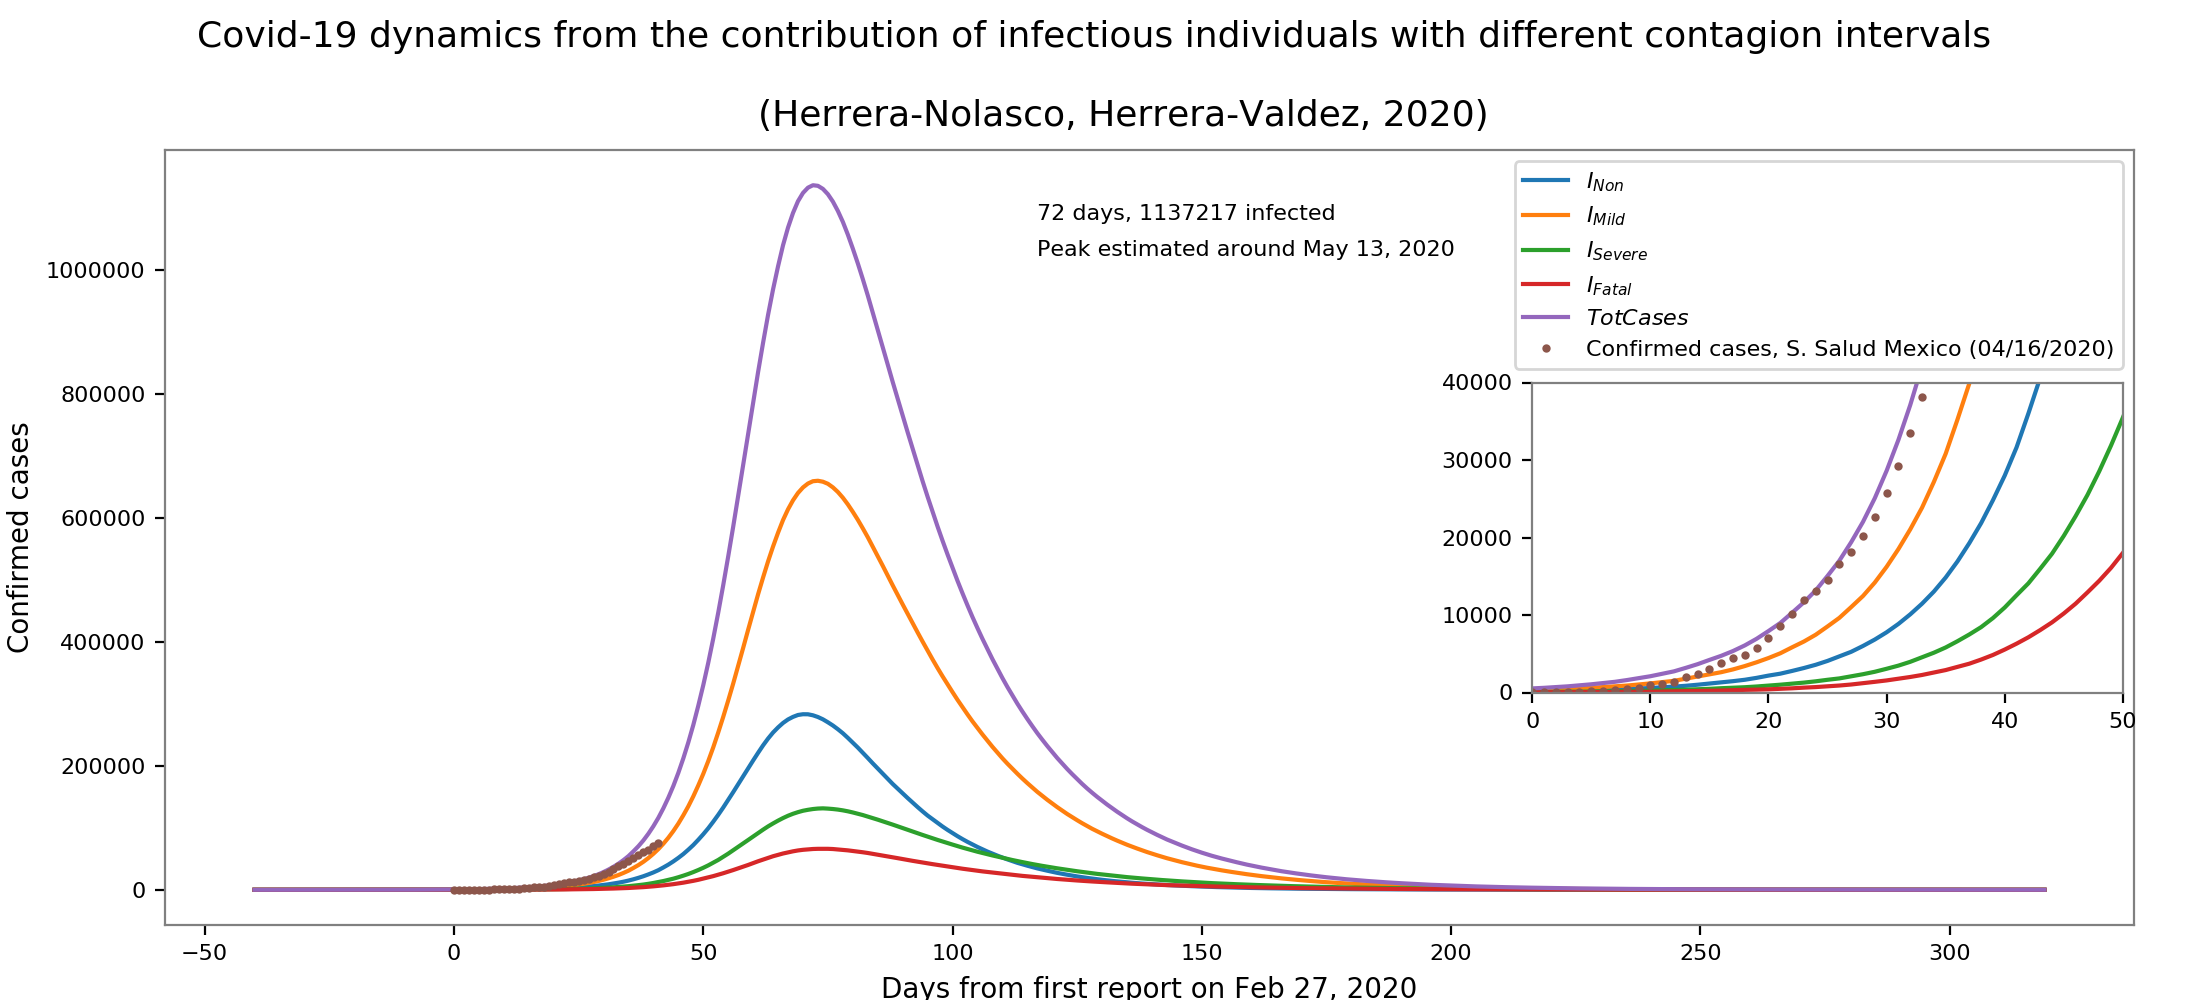
\includegraphics[width=\textwidth]{figures/Covid19_Mexico_InitialFit_Herrera-Valdez+Herrera-Nolasco_2020}
\caption{Estimación de la fecha de inicio y pico de la epidemia ajustando los datos iniciales de la epidemia de Covid-19 en México. La fecha cero representa el 27 de febrero de 2020. Para estas simulaciones los infectados de los grupos severo y crítico en las simulaciones tienen exposición nula a otros grupos poblacionales. } \label{fig:inicioPicoNIW}
\end{figure}

Explicitamente,
\begin{eqnarray}
N(t+h) &=& N(t) - X(t)
 \label{eq:N} \\
I(t+h) &=& X(t) - Y(t)
\label{eq:I}\\
W(t+h) &=& W(t) + Y(t) - D(t)
\label{eq:W}
\end{eqnarray}
donde $X(t)$, $Y(t)$, y $D(t)$ son variables aleatorias entera que representan, respectivamente, la incidencia de infección, los nuevos casos removidos del la cadena de infección al cumplir su periodo infeccioso (recuperados), y los nuevos fallecidos. Los miembros del grupo $W$ ya no participan en la cadena de transmisión. El total poblacional $N+I+T$ no es constante. La dinámica de la epidemia está supuesta como un proceso estocástico no homogéneo en el que no necesariamente hay mezcla homogénea entre infectados y no infectados. Para fines computacionales, las simulaciones están basadas en muestreos binomiales o Poisson, dependiendo de la cantidad de ensayos requeridos en cada muestreo.

 La probabilidad de éxito para cada muestreo puede depender de la cantidad de infectados y su posible contribución (por exposición) a la cadena de transmisión (para $X$), o de tiempos de recuperación y posiblemente muerte (para $Y$). El modelo mostrado en las ecuaciones \eqref{eq:N}-\eqref{eq:W} también permite simular dinámicas epidémicas en poblaciones pequeñas, y controlar de forma independiente  factores como la exposición de los susceptibles al contagio y la contribución de los infectados de distintos grupos, lo que permite considerar escenarios de distanciamiento social, aislamiento de casos sospechosos, aislamiento de casos y la posible contribución de grupos de individuos asintomáticos.


 Por el momento, hemos encontrado regímenes de parámetros al rededor de los cuales podemos simular la dinámica macroscópica de la epidemia en México ajustada con los datos de la Secretaría de Salud de México (\figref{fig:inicioPicoNIW}). Por construcción, sólo una proporción de los susceptibles y una proporción de los infectados están en contacto. Con el fin de dar estimaciones conservadoras de inicio, hemos realizado simulaciones en las que la exposición de susceptibles al contagio es constante, ajustando los datos de la Secretaría de salud  con un factor de 12, y  suponiendo una  población expuesta al 10\%. En esas condiciones, una estimación \textit{conservadora} de la fecha de inicio de la epidemia es aproximadamente 40 días antes del 27 de febrero. Es decir, aproximadamente el 20 de enero de 2020. El pico de la infección estaría estimado para ocurrir al rededor de 75 días después del día 0. Es decir, al rededor de Mayo 14 de 2020. La tendencia de los datos de los últimos días es de crecimiento menor en comparación a las simulaciones. Esto indica que posiblemente haya un retraso aún mayor para observar el pico de la epidemia y con un número de casos menor.

En esta dirección, ha resultado útil un caso particular del modelo en las ecuaciones \eqref{eq:N}-\eqref{eq:W}  para explorar escenarios en grandes números.
 Para ello, tomamos los valores esperados de los muestreos del modelo estocástico y derivamos una ecuación determinista para el régimen en el que los tamaños poblacionales son grandes (\figref{fig:inicioPicoNIW}). Como resultado obtenemos un modelo que tiene similitud con un SIR clásico.

\bigskip
\begin{minipage}{0.6\textwidth}
De forma explícita, si el tamaño de la población $T=N+I+W$ considerada en el sistema \eqref{eq:N}-\eqref{eq:W} es lo suficientemente grande, es posible derivar un sistema de ecuaciones diferenciales ordinarias para las densidades poblacionales de no-infectados, infectados y removidos, representadas por $x$, $\vec{y}$, y $w$, de tal forma que
\begin{eqnarray*}
\partial_{t} x &=& -  \lambda x\\
\partial_{t} y &=& \lambda x - \vec{\gamma} \cdot \vec{y}  - \delta_{F} y_{C}
\\
\partial_{t} w &=&\vec{\gamma} \cdot \vec{y} + \delta_{F} y_{C}
\end{eqnarray*}
donde $\vec{y}$ y  $\vec{\gamma}$  son  vectores que representan, respectivamente,  los tamaños de la subpoblaciones infecciosas y las tasas de remoción para cada grupo infeccioso. La variable $y$ representa la prevalencia (puntual) de infecciones en la población en el tiempo $t$.
\end{minipage}%
\begin{minipage}{0.4\textwidth}
\centering
\begin{tikzpicture}[scale=0.6,transform shape]
	\vertex[label=\textcolor{black}{$N$},color=black](N) at (-4,0) { };
	\vertex[label=\textcolor{black}{$I_{A}$},color=red](A) at (0,3) {};
	\vertex[label=\textcolor{black}{$I_{M}$},color=red](M) at (0,1) {};
	\vertex[label=\textcolor{black}{$I_{S}$},color=red](S) at (0,-1) {};
	\vertex[label=\textcolor{black}{$I_{C}$},color=red](C) at (0,-3) {};
	\vertex[label=\textcolor{black}{$W$},color=black](W) at (4,0) { };
	\vertex[label=\textcolor{black}{$F$}](F) at (3,-3) {};
  \tikzstyle{LabelStyle}=[fill=white,sloped]
  \tikzstyle{EdgeStyle}=[bend left]
  \Edge[label=$\lambda_{A}$,color=red](N)(A)
  \Edge[label=$\lambda_{M}$,color=red](N)(M)
  \Edge[label=$\beta_{AW}$,color=blue](A)(W)
  \Edge[label=$\beta_{MW}$,color=blue](M)(W)
  \tikzstyle{EdgeStyle}=[bend right]
  \Edge[label=$\lambda_{S}$,color=red](N)(S)
  \Edge[label=$\lambda_{C}$,color=red](N)(C)
  \Edge[label=$\beta_{SW}$,color=blue](S)(W)
  \Edge[label=$\beta_{CW}$,color=blue](C)(W)
  \Edge[label=$\gamma_{CF}$](C)(F)
\end{tikzpicture}
\end{minipage}%



\subsubsection*{Trabajo en progreso.} Continuamos desarrollando modelos estocásticos de dinámica de propagación basados en estimaciones cualitativas similares a las descritas arriba, basadas en tendencias observadas en otros países del mundo, con la intención de explicar mecanismos subyacentes a la propagación de la epidemia, y también para fines de contraste con la situación de México, en caso de tener datos disponibles para hacer comparaciones.
 En particular, estamos desarrollando modelos que nos permitan considerar estadíos clínicos de la enfermedad y tomar en cuenta la patofisiología asociada a la infección causada por SARS-Cov-2.
